\documentclass[twoside]{book}

% Packages required by doxygen
\usepackage{fixltx2e}
\usepackage{calc}
\usepackage{doxygen}
\usepackage[export]{adjustbox} % also loads graphicx
\usepackage{graphicx}
\usepackage[utf8]{inputenc}
\usepackage{makeidx}
\usepackage{multicol}
\usepackage{multirow}
\PassOptionsToPackage{warn}{textcomp}
\usepackage{textcomp}
\usepackage[nointegrals]{wasysym}
\usepackage[table]{xcolor}

% Font selection
\usepackage[T1]{fontenc}
\usepackage[scaled=.90]{helvet}
\usepackage{courier}
\usepackage{amssymb}
\usepackage{sectsty}
\renewcommand{\familydefault}{\sfdefault}
\allsectionsfont{%
  \fontseries{bc}\selectfont%
  \color{darkgray}%
}
\renewcommand{\DoxyLabelFont}{%
  \fontseries{bc}\selectfont%
  \color{darkgray}%
}
\newcommand{\+}{\discretionary{\mbox{\scriptsize$\hookleftarrow$}}{}{}}

% Page & text layout
\usepackage{geometry}
\geometry{%
  a4paper,%
  top=2.5cm,%
  bottom=2.5cm,%
  left=2.5cm,%
  right=2.5cm%
}
\tolerance=750
\hfuzz=15pt
\hbadness=750
\setlength{\emergencystretch}{15pt}
\setlength{\parindent}{0cm}
\setlength{\parskip}{3ex plus 2ex minus 2ex}
\makeatletter
\renewcommand{\paragraph}{%
  \@startsection{paragraph}{4}{0ex}{-1.0ex}{1.0ex}{%
    \normalfont\normalsize\bfseries\SS@parafont%
  }%
}
\renewcommand{\subparagraph}{%
  \@startsection{subparagraph}{5}{0ex}{-1.0ex}{1.0ex}{%
    \normalfont\normalsize\bfseries\SS@subparafont%
  }%
}
\makeatother

% Headers & footers
\usepackage{fancyhdr}
\pagestyle{fancyplain}
\fancyhead[LE]{\fancyplain{}{\bfseries\thepage}}
\fancyhead[CE]{\fancyplain{}{}}
\fancyhead[RE]{\fancyplain{}{\bfseries\leftmark}}
\fancyhead[LO]{\fancyplain{}{\bfseries\rightmark}}
\fancyhead[CO]{\fancyplain{}{}}
\fancyhead[RO]{\fancyplain{}{\bfseries\thepage}}
\fancyfoot[LE]{\fancyplain{}{}}
\fancyfoot[CE]{\fancyplain{}{}}
\fancyfoot[RE]{\fancyplain{}{\bfseries\scriptsize Generated by Doxygen }}
\fancyfoot[LO]{\fancyplain{}{\bfseries\scriptsize Generated by Doxygen }}
\fancyfoot[CO]{\fancyplain{}{}}
\fancyfoot[RO]{\fancyplain{}{}}
\renewcommand{\footrulewidth}{0.4pt}
\renewcommand{\chaptermark}[1]{%
  \markboth{#1}{}%
}
\renewcommand{\sectionmark}[1]{%
  \markright{\thesection\ #1}%
}

% Indices & bibliography
\usepackage{natbib}
\usepackage[titles]{tocloft}
\setcounter{tocdepth}{3}
\setcounter{secnumdepth}{5}
\makeindex

% Hyperlinks (required, but should be loaded last)
\usepackage{ifpdf}
\ifpdf
  \usepackage[pdftex,pagebackref=true]{hyperref}
\else
  \usepackage[ps2pdf,pagebackref=true]{hyperref}
\fi
\hypersetup{%
  colorlinks=true,%
  linkcolor=blue,%
  citecolor=blue,%
  unicode%
}

% Custom commands
\newcommand{\clearemptydoublepage}{%
  \newpage{\pagestyle{empty}\cleardoublepage}%
}

\usepackage{caption}
\captionsetup{labelsep=space,justification=centering,font={bf},singlelinecheck=off,skip=4pt,position=top}

%===== C O N T E N T S =====

\begin{document}

% Titlepage & ToC
\hypersetup{pageanchor=false,
             bookmarksnumbered=true,
             pdfencoding=unicode
            }
\pagenumbering{alph}
\begin{titlepage}
\vspace*{7cm}
\begin{center}%
{\Large My Project }\\
\vspace*{1cm}
{\large Generated by Doxygen 1.8.13}\\
\end{center}
\end{titlepage}
\clearemptydoublepage
\pagenumbering{roman}
\tableofcontents
\clearemptydoublepage
\pagenumbering{arabic}
\hypersetup{pageanchor=true}

%--- Begin generated contents ---
\chapter{Project 5 -\/ Numerical Integration}
\label{md_README}
\Hypertarget{md_README}
\input{md_README}
\chapter{Hierarchical Index}
\section{Class Hierarchy}
This inheritance list is sorted roughly, but not completely, alphabetically\+:\begin{DoxyCompactList}
\item \contentsline{section}{Abstract\+Integration\+Method}{\pageref{class_abstract_integration_method}}{}
\begin{DoxyCompactList}
\item \contentsline{section}{Midpoint\+Formula}{\pageref{class_midpoint_formula}}{}
\item \contentsline{section}{Simpsons\+Rule}{\pageref{class_simpsons_rule}}{}
\item \contentsline{section}{Trapezoidal\+Rule}{\pageref{class_trapezoidal_rule}}{}
\end{DoxyCompactList}
\item \contentsline{section}{Abstract\+Reader}{\pageref{class_abstract_reader}}{}
\begin{DoxyCompactList}
\item \contentsline{section}{Txt\+Reader}{\pageref{class_txt_reader}}{}
\end{DoxyCompactList}
\item \contentsline{section}{Data}{\pageref{struct_data}}{}
\end{DoxyCompactList}

\chapter{Class Index}
\section{Class List}
Here are the classes, structs, unions and interfaces with brief descriptions\+:\begin{DoxyCompactList}
\item\contentsline{section}{\hyperlink{class_abstract_integration_method}{Abstract\+Integration\+Method} \\*Abstract class for implementation of integration algorithms }{\pageref{class_abstract_integration_method}}{}
\item\contentsline{section}{\hyperlink{class_abstract_reader}{Abstract\+Reader} \\*Abstract class for implementation of file reading }{\pageref{class_abstract_reader}}{}
\item\contentsline{section}{\hyperlink{struct_data}{Data} \\*Struct storing data for the integral computation }{\pageref{struct_data}}{}
\item\contentsline{section}{\hyperlink{class_midpoint_formula}{Midpoint\+Formula} \\*Class implementing the Midpoint Formula approximation of integrals in 2D or 1D }{\pageref{class_midpoint_formula}}{}
\item\contentsline{section}{\hyperlink{class_simpsons_rule}{Simpsons\+Rule} \\*Class implementing the Simpson\textquotesingle{}s Rule approximation of integrals in 2D or 1D }{\pageref{class_simpsons_rule}}{}
\item\contentsline{section}{\hyperlink{class_trapezoidal_rule}{Trapezoidal\+Rule} \\*Class implementing the Trapezoidal Rule approximation of integrals in 2D or 1D }{\pageref{class_trapezoidal_rule}}{}
\item\contentsline{section}{\hyperlink{class_txt_reader}{Txt\+Reader} \\*Class implementing reading data from T\+XT riles }{\pageref{class_txt_reader}}{}
\end{DoxyCompactList}

\chapter{Class Documentation}
\hypertarget{classAbstractIntegrationMethod}{}\section{Abstract\+Integration\+Method Class Reference}
\label{classAbstractIntegrationMethod}\index{Abstract\+Integration\+Method@{Abstract\+Integration\+Method}}


Inheritance diagram for Abstract\+Integration\+Method\+:
\nopagebreak
\begin{figure}[H]
\begin{center}
\leavevmode
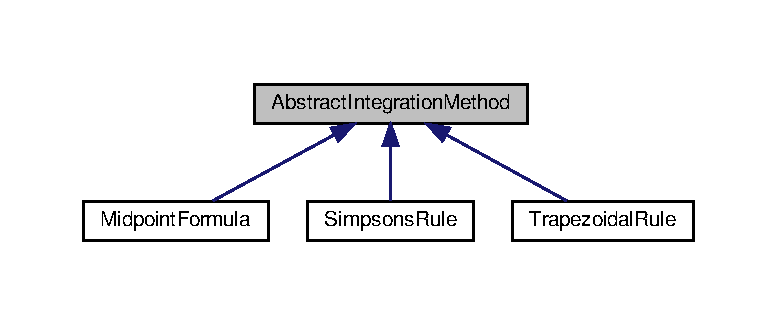
\includegraphics[width=350pt]{classAbstractIntegrationMethod__inherit__graph}
\end{center}
\end{figure}


Collaboration diagram for Abstract\+Integration\+Method\+:
\nopagebreak
\begin{figure}[H]
\begin{center}
\leavevmode
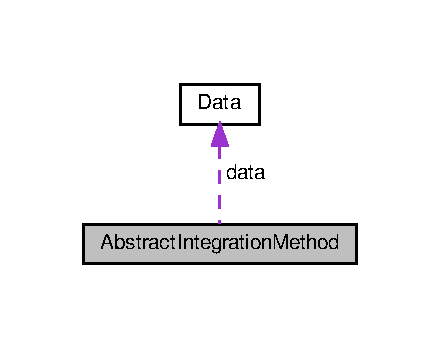
\includegraphics[width=211pt]{classAbstractIntegrationMethod__coll__graph}
\end{center}
\end{figure}
\subsection*{Public Member Functions}
\begin{DoxyCompactItemize}
\item 
\mbox{\Hypertarget{classAbstractIntegrationMethod_a2b3a0208c99564d496e27b383fc4d96f}\label{classAbstractIntegrationMethod_a2b3a0208c99564d496e27b383fc4d96f}} 
{\bfseries Abstract\+Integration\+Method} (\hyperlink{structData}{Data} data, Eigen\+::\+Vector\+Xcd($\ast$function)(double x, double y, Eigen\+::\+Matrix\+Xcd coeff))
\item 
\mbox{\Hypertarget{classAbstractIntegrationMethod_af76e5bdce7d0b139d07e920fa29c1c34}\label{classAbstractIntegrationMethod_af76e5bdce7d0b139d07e920fa29c1c34}} 
virtual Eigen\+::\+Vector\+Xcd {\bfseries Solve} ()=0
\end{DoxyCompactItemize}
\subsection*{Protected Attributes}
\begin{DoxyCompactItemize}
\item 
\mbox{\Hypertarget{classAbstractIntegrationMethod_a534b5ff7dfbccc1332cfbe66e817b389}\label{classAbstractIntegrationMethod_a534b5ff7dfbccc1332cfbe66e817b389}} 
\hyperlink{structData}{Data} {\bfseries data}
\item 
\mbox{\Hypertarget{classAbstractIntegrationMethod_a4de4f7ee55737b4f05f2b02649bf5ea0}\label{classAbstractIntegrationMethod_a4de4f7ee55737b4f05f2b02649bf5ea0}} 
Eigen\+::\+Vector\+Xcd($\ast$ {\bfseries f} )(double x, double y, Eigen\+::\+Matrix\+Xcd coeff)
\end{DoxyCompactItemize}


The documentation for this class was generated from the following files\+:\begin{DoxyCompactItemize}
\item 
Abstract\+Integration\+Method.\+h\item 
Abstract\+Integration\+Method.\+cpp\end{DoxyCompactItemize}

\hypertarget{classAbstractReader}{}\section{Abstract\+Reader Class Reference}
\label{classAbstractReader}\index{Abstract\+Reader@{Abstract\+Reader}}


Inheritance diagram for Abstract\+Reader\+:
\nopagebreak
\begin{figure}[H]
\begin{center}
\leavevmode
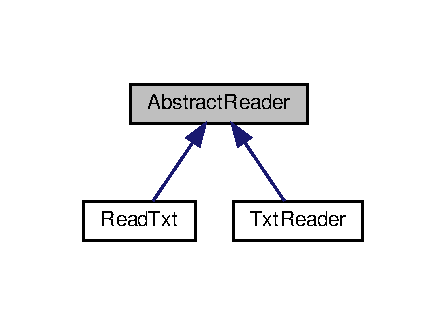
\includegraphics[width=214pt]{classAbstractReader__inherit__graph}
\end{center}
\end{figure}
\subsection*{Public Member Functions}
\begin{DoxyCompactItemize}
\item 
\mbox{\Hypertarget{classAbstractReader_af7d4391a1d75538c6bb406c00acabd30}\label{classAbstractReader_af7d4391a1d75538c6bb406c00acabd30}} 
{\bfseries Abstract\+Reader} (std\+::string filename)
\item 
\mbox{\Hypertarget{classAbstractReader_a14b05f156920be0cfa0cabdb1c6c1267}\label{classAbstractReader_a14b05f156920be0cfa0cabdb1c6c1267}} 
virtual \hyperlink{structData}{Data} {\bfseries Output\+Data} ()=0
\end{DoxyCompactItemize}
\subsection*{Protected Attributes}
\begin{DoxyCompactItemize}
\item 
\mbox{\Hypertarget{classAbstractReader_a143f9961ba8aca61c32234a042e466ce}\label{classAbstractReader_a143f9961ba8aca61c32234a042e466ce}} 
std\+::string {\bfseries fname}
\end{DoxyCompactItemize}


The documentation for this class was generated from the following files\+:\begin{DoxyCompactItemize}
\item 
Abstract\+Reader.\+h\item 
Abstract\+Reader.\+cpp\end{DoxyCompactItemize}

\hypertarget{structData}{}\section{Data Struct Reference}
\label{structData}\index{Data@{Data}}
\subsection*{Public Attributes}
\begin{DoxyCompactItemize}
\item 
\mbox{\Hypertarget{structData_a5d52cb2b68c752fa8b74b86ccb1d7e3d}\label{structData_a5d52cb2b68c752fa8b74b86ccb1d7e3d}} 
Eigen\+::\+Matrix\+X2d {\bfseries boundsX}
\item 
\mbox{\Hypertarget{structData_aa34a405b70244ad387719f8d38de51ed}\label{structData_aa34a405b70244ad387719f8d38de51ed}} 
Eigen\+::\+Matrix\+X2d {\bfseries boundsY}
\item 
\mbox{\Hypertarget{structData_a97a70b84170c9d1e46705fc5a8e1db20}\label{structData_a97a70b84170c9d1e46705fc5a8e1db20}} 
Eigen\+::\+Matrix\+X2i {\bfseries no\+Steps}
\item 
\mbox{\Hypertarget{structData_aa8aaf26f991decdf85559d5fa417f520}\label{structData_aa8aaf26f991decdf85559d5fa417f520}} 
Eigen\+::\+Matrix\+Xcd {\bfseries coefficients}
\item 
\mbox{\Hypertarget{structData_afe887f8ffbf8e145e0277093134cabcc}\label{structData_afe887f8ffbf8e145e0277093134cabcc}} 
int {\bfseries D}
\item 
\mbox{\Hypertarget{structData_ab256a1176f3ba99a220c648b0c855840}\label{structData_ab256a1176f3ba99a220c648b0c855840}} 
int {\bfseries m}
\end{DoxyCompactItemize}


The documentation for this struct was generated from the following file\+:\begin{DoxyCompactItemize}
\item 
Data\+Struct.\+h\end{DoxyCompactItemize}

\hypertarget{classMidpointFormula}{}\section{Midpoint\+Formula Class Reference}
\label{classMidpointFormula}\index{Midpoint\+Formula@{Midpoint\+Formula}}


Inheritance diagram for Midpoint\+Formula\+:\nopagebreak
\begin{figure}[H]
\begin{center}
\leavevmode
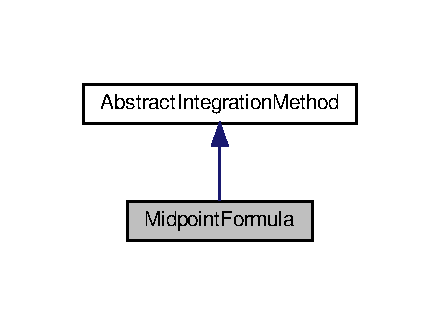
\includegraphics[width=211pt]{classMidpointFormula__inherit__graph}
\end{center}
\end{figure}


Collaboration diagram for Midpoint\+Formula\+:\nopagebreak
\begin{figure}[H]
\begin{center}
\leavevmode
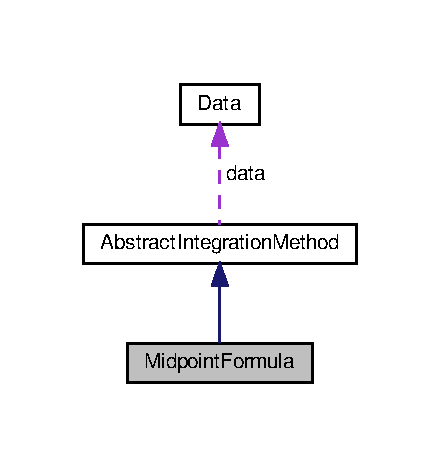
\includegraphics[width=211pt]{classMidpointFormula__coll__graph}
\end{center}
\end{figure}
\subsection*{Public Member Functions}
\begin{DoxyCompactItemize}
\item 
\mbox{\Hypertarget{classMidpointFormula_ad3c444776b53996d50dbf88a61c36c8c}\label{classMidpointFormula_ad3c444776b53996d50dbf88a61c36c8c}} 
{\bfseries Midpoint\+Formula} (\hyperlink{structData}{Data} data, Eigen\+::\+Vector\+Xcd($\ast$f)(double x, double y, Eigen\+::\+Matrix\+Xcd coeff))
\item 
\mbox{\Hypertarget{classMidpointFormula_add437323dfb0bc181b0051c5aaf80ba7}\label{classMidpointFormula_add437323dfb0bc181b0051c5aaf80ba7}} 
Eigen\+::\+Vector\+Xcd {\bfseries Solve} ()
\end{DoxyCompactItemize}
\subsection*{Additional Inherited Members}


The documentation for this class was generated from the following files\+:\begin{DoxyCompactItemize}
\item 
Midpoint\+Formula.\+h\item 
Midpoint\+Formula.\+cpp\end{DoxyCompactItemize}

\hypertarget{classReadTxt}{}\section{Read\+Txt Class Reference}
\label{classReadTxt}\index{Read\+Txt@{Read\+Txt}}


Inheritance diagram for Read\+Txt\+:
\nopagebreak
\begin{figure}[H]
\begin{center}
\leavevmode
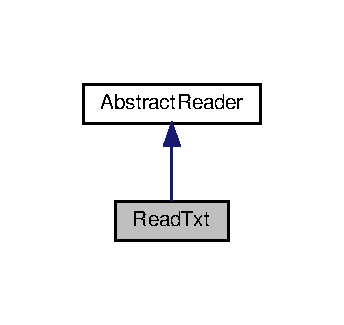
\includegraphics[width=165pt]{classReadTxt__inherit__graph}
\end{center}
\end{figure}


Collaboration diagram for Read\+Txt\+:
\nopagebreak
\begin{figure}[H]
\begin{center}
\leavevmode
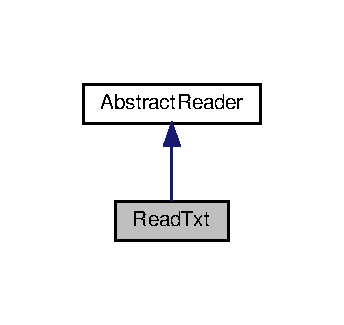
\includegraphics[width=165pt]{classReadTxt__coll__graph}
\end{center}
\end{figure}
\subsection*{Public Member Functions}
\begin{DoxyCompactItemize}
\item 
\mbox{\Hypertarget{classReadTxt_af66a9abde28671c08264b28c26646c2a}\label{classReadTxt_af66a9abde28671c08264b28c26646c2a}} 
{\bfseries Read\+Txt} (const string \&fname)
\item 
\mbox{\Hypertarget{classReadTxt_adee9ad45d93fce109d24edaaa834a568}\label{classReadTxt_adee9ad45d93fce109d24edaaa834a568}} 
\hyperlink{structData}{Data} {\bfseries read\+Txt} ()
\end{DoxyCompactItemize}
\subsection*{Additional Inherited Members}


The documentation for this class was generated from the following files\+:\begin{DoxyCompactItemize}
\item 
offreadfile.\+h\item 
offreadfile.\+cpp\end{DoxyCompactItemize}

\hypertarget{classSimpsonsRule}{}\section{Simpsons\+Rule Class Reference}
\label{classSimpsonsRule}\index{Simpsons\+Rule@{Simpsons\+Rule}}


Inheritance diagram for Simpsons\+Rule\+:\nopagebreak
\begin{figure}[H]
\begin{center}
\leavevmode
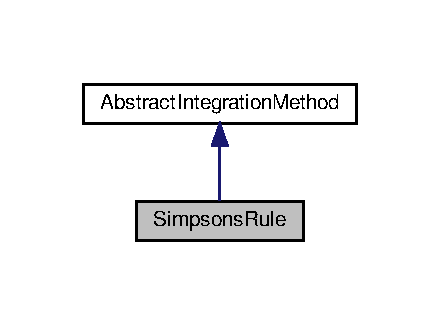
\includegraphics[width=211pt]{classSimpsonsRule__inherit__graph}
\end{center}
\end{figure}


Collaboration diagram for Simpsons\+Rule\+:\nopagebreak
\begin{figure}[H]
\begin{center}
\leavevmode
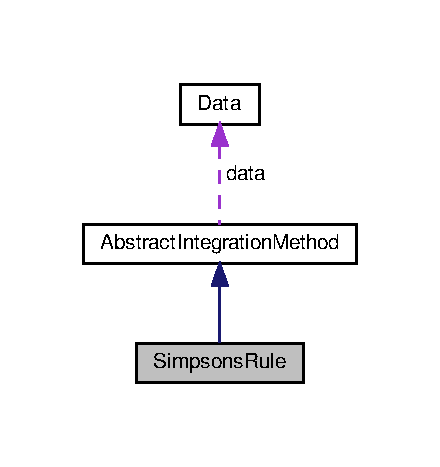
\includegraphics[width=211pt]{classSimpsonsRule__coll__graph}
\end{center}
\end{figure}
\subsection*{Public Member Functions}
\begin{DoxyCompactItemize}
\item 
\mbox{\Hypertarget{classSimpsonsRule_af880433d19d6041cdedb081b542a195b}\label{classSimpsonsRule_af880433d19d6041cdedb081b542a195b}} 
{\bfseries Simpsons\+Rule} (\hyperlink{structData}{Data} data, Eigen\+::\+Vector\+Xcd($\ast$f)(double x, double y, Eigen\+::\+Matrix\+Xcd coeff))
\item 
\mbox{\Hypertarget{classSimpsonsRule_a9925b07e44be9fc1644d3cbeb742078c}\label{classSimpsonsRule_a9925b07e44be9fc1644d3cbeb742078c}} 
Eigen\+::\+Vector\+Xcd {\bfseries Solve} ()
\end{DoxyCompactItemize}
\subsection*{Additional Inherited Members}


The documentation for this class was generated from the following files\+:\begin{DoxyCompactItemize}
\item 
Simpsons\+Rule.\+h\item 
Simpsons\+Rule.\+cpp\end{DoxyCompactItemize}

\hypertarget{classTrapezoidalRule}{}\section{Trapezoidal\+Rule Class Reference}
\label{classTrapezoidalRule}\index{Trapezoidal\+Rule@{Trapezoidal\+Rule}}


Inheritance diagram for Trapezoidal\+Rule\+:
\nopagebreak
\begin{figure}[H]
\begin{center}
\leavevmode
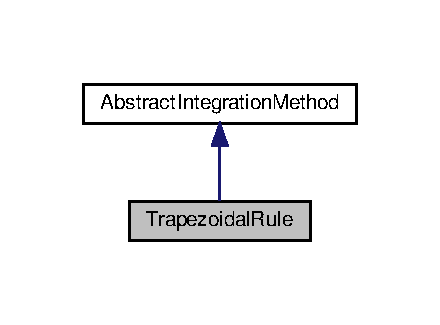
\includegraphics[width=211pt]{classTrapezoidalRule__inherit__graph}
\end{center}
\end{figure}


Collaboration diagram for Trapezoidal\+Rule\+:
\nopagebreak
\begin{figure}[H]
\begin{center}
\leavevmode
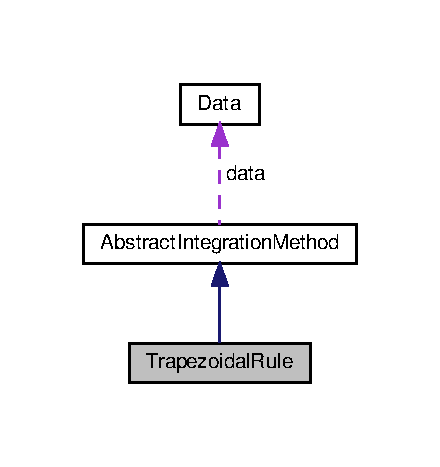
\includegraphics[width=211pt]{classTrapezoidalRule__coll__graph}
\end{center}
\end{figure}
\subsection*{Public Member Functions}
\begin{DoxyCompactItemize}
\item 
\mbox{\Hypertarget{classTrapezoidalRule_ac366b3b5a8758ad00590f029c0b0bdd7}\label{classTrapezoidalRule_ac366b3b5a8758ad00590f029c0b0bdd7}} 
{\bfseries Trapezoidal\+Rule} (\hyperlink{structData}{Data} data, Eigen\+::\+Vector\+Xcd($\ast$f)(double x, double y, Eigen\+::\+Matrix\+Xcd coeff))
\item 
\mbox{\Hypertarget{classTrapezoidalRule_ae822d86948bdc8876bf524cd620e11b8}\label{classTrapezoidalRule_ae822d86948bdc8876bf524cd620e11b8}} 
Eigen\+::\+Vector\+Xcd {\bfseries Solve} ()
\end{DoxyCompactItemize}
\subsection*{Additional Inherited Members}


The documentation for this class was generated from the following files\+:\begin{DoxyCompactItemize}
\item 
Trapezoidal\+Rule.\+h\item 
Trapezoidal\+Rule.\+cpp\end{DoxyCompactItemize}

\hypertarget{classTxtReader}{}\section{Txt\+Reader Class Reference}
\label{classTxtReader}\index{Txt\+Reader@{Txt\+Reader}}


Inheritance diagram for Txt\+Reader\+:\nopagebreak
\begin{figure}[H]
\begin{center}
\leavevmode
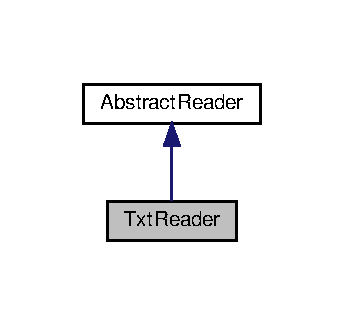
\includegraphics[width=165pt]{classTxtReader__inherit__graph}
\end{center}
\end{figure}


Collaboration diagram for Txt\+Reader\+:\nopagebreak
\begin{figure}[H]
\begin{center}
\leavevmode
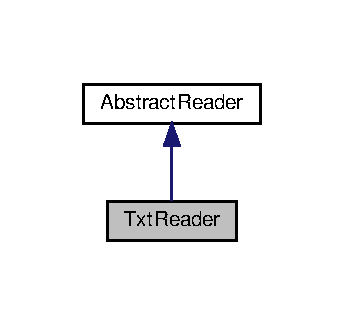
\includegraphics[width=165pt]{classTxtReader__coll__graph}
\end{center}
\end{figure}
\subsection*{Public Member Functions}
\begin{DoxyCompactItemize}
\item 
\mbox{\Hypertarget{classTxtReader_acbef0ef9c6034581d76a3b9e305f1508}\label{classTxtReader_acbef0ef9c6034581d76a3b9e305f1508}} 
{\bfseries Txt\+Reader} (std\+::string filename)
\item 
\mbox{\Hypertarget{classTxtReader_a30786dcd83c2f24dd26e83cb5fd934ab}\label{classTxtReader_a30786dcd83c2f24dd26e83cb5fd934ab}} 
\hyperlink{structData}{Data} {\bfseries Output\+Data} ()
\end{DoxyCompactItemize}
\subsection*{Additional Inherited Members}


The documentation for this class was generated from the following files\+:\begin{DoxyCompactItemize}
\item 
Txt\+Reader.\+h\item 
Txt\+Reader.\+cpp\end{DoxyCompactItemize}

%--- End generated contents ---

% Index
\backmatter
\newpage
\phantomsection
\clearemptydoublepage
\addcontentsline{toc}{chapter}{Index}
\printindex

\end{document}
